\documentclass[conference]{IEEEtran}
\IEEEoverridecommandlockouts

\usepackage[T1]{fontenc}
\usepackage{cite}
\usepackage{amsmath,amssymb,amsfonts}
\usepackage{algorithmic}
\usepackage{graphicx}
\usepackage{textcomp}
\usepackage{xcolor}
\usepackage{microtype}
\usepackage{array}
\usepackage{booktabs}
\usepackage{placeins}
\newcolumntype{L}[1]{>{\raggedright\arraybackslash}p{#1}}
\newcolumntype{C}[1]{>{\centering\arraybackslash}p{#1}}
\emergencystretch=2em

\def\BibTeX{{\rm B\kern-.05em{\sc i\kern-.025em b}\kern-.08em
    T\kern-.1667em\lower.7ex\hbox{E}\kern-.125emX}}

\title{Analyzing Modern Activation Functions to Optimize\\
Gated Recurrent Networks for Sentiment Classification}

% Double-blind submission: Authors are anonymized for the initial review.
\author{\IEEEauthorblockN{Anonymous Authors}}

\begin{document}
\raggedbottom

\maketitle

\begin{abstract}
This study measures how the choice of activation function in
the dense layers of gated recurrent networks affects sentiment
classification on the IMDb movie review dataset. LSTM and GRU
networks are standard for this task, but the activation
functions in the dense layers after the recurrent part are rarely
studied. We test all 100 ordered pairs of ten activation functions,
covering both classical functions and the modern smooth family
(GELU, SiLU, Mish, and others), across four architectures: LSTM,
GRU, and the fully bidirectional version of each, for 400 models
in total, with every other setting held fixed. All ten of the best
configurations use GRU, and GRU tolerates a poor activation
choice better than LSTM. The best activation for one architecture
is often the worst for another, so rankings do not transfer
between cell types. A separate convergence test shows that smooth
activations reach up to 81\% validation accuracy after a single
epoch, compared to 64\% for ReLU, though all functions converge
to similar accuracy within three epochs. We also document an
architecture-specific dead-neuron failure when ReLU is used
in the dense layers of an LSTM. Together these results give
concrete guidance on which activation to use, where, and in
which architecture.
\end{abstract}

\begin{IEEEkeywords}
Sentiment Analysis, IMDb Dataset, Deep Learning, LSTM, GRU, Activation Functions, GELU, Mish, Natural Language Processing.
\end{IEEEkeywords}

\section{Introduction}

Sentiment analysis is the task of deciding whether a piece of
text is positive or negative. It is one of the most common
problems in natural language processing. The IMDb Large
Movie Review Dataset, with 50{,}000 balanced reviews, is the
standard benchmark for the binary version of the
task~\cite{maas2011}. LSTM and GRU networks are the usual
choice for this problem because their gating mechanisms let
them track context across long sequences~\cite{hochreiter1997,cho2014,chung2014}.

One part of these models gets little attention: the activation
function in the dense layers that sit after the recurrent
layers. The gates inside the recurrent cell are fixed to
sigmoid and tanh, but the dense layers that turn the recurrent
output into a final prediction can use any activation function.
Ahmed et al.~\cite{ahmed2025} tested three classical
combinations in a bidirectional LSTM, reached 88.40\% accuracy,
and asked for follow-up work on modern activation functions and
other architectures. This study does that.

We test all 100 ordered pairs of ten activation functions
across four architectures (LSTM, GRU, and the fully
bidirectional version of each), for 400 models in total. Every
other setting is held fixed, so the activation pair is the only
thing that changes. We use this setup to answer six questions:

\begin{itemize}
  \item \textbf{RQ1:} Which activation pair gives the highest test accuracy?
  \item \textbf{RQ2:} Which activations converge fastest?
  \item \textbf{RQ3:} Which activation pair produces the most balanced predictions?
  \item \textbf{RQ4:} Do GRU and LSTM respond differently to activation changes?
  \item \textbf{RQ5:} Do non-saturating activations improve gradient flow over Tanh?
  \item \textbf{RQ6:} Do ReLU-based dense layers cause dead-neuron problems?
\end{itemize}

\FloatBarrier
\section{Literature Review}

Hochreiter and Schmidhuber~\cite{hochreiter1997} introduced
the LSTM to solve the vanishing gradient problem in recurrent
networks, using sigmoid and tanh as internal gate activations.
Cho et al.~\cite{cho2014} proposed the GRU, which reduces the gating
structure to two gates and merges the cell and hidden states, and Chung
et al.~\cite{chung2014} showed that GRU matches LSTM on sequence
tasks with fewer parameters. Schuster and Paliwal~\cite{schuster1997}
added bidirectionality, letting the model use both past and future
context. None of these works asked whether the activation
functions in the layers around the recurrent cells were optimal.

The activation function literature evolved separately. Nair
and Hinton~\cite{nair2010} introduced ReLU and showed that avoiding
saturation improves gradient flow, though at the cost of
killing neurons that receive negative inputs. Maas et al.~\cite{maas2013}
addressed this with LeakyReLU, and Clevert et al.~\cite{clevert2015} with
ELU, whose smooth negative region avoids the dead-neuron
problem. Klambauer et al.~\cite{klambauer2017} introduced SELU with a
self-normalising property under specific initialization. More recently,
GELU~\cite{hendrycks2016} became the default in transformers, Swish~\cite{ramachandran2017} was
found through automated search, and Mish~\cite{misra2020} outperformed
both on vision benchmarks. Surveys by Nwankpa et al.~\cite{nwankpa2018}
and Apicella et al.~\cite{apicella2021} catalogue the growing range of
trainable activation functions. All of these were developed and
tested in feedforward, convolutional, or transformer settings.
Their behaviour inside gated recurrent dense layers remained
untested.

Within sentiment analysis, the IMDb dataset~\cite{maas2011} is the
standard benchmark for binary classification. Tang et al.~\cite{tang2015}
validated GRU for document-level sentiment and Socher et
al.~\cite{socher2013} contributed the SST treebank. Several studies addressed
the activation question partially. Eger et al.~\cite{eger2018} compared 21
activations across NLP tasks but used basic architectures and
predated widespread use of Mish. Farzad et al.~\cite{farzad2019} swept 23
functions at the LSTM gate level on IMDb but tested no GRU
or bidirectional variants. Essai Ali et al.~\cite{essaiAli2022} engineered 26
novel activations for LSTM but outside sentiment and without
GELU, Swish, or Mish. Zhu and Tan~\cite{zhu2022} tested a custom
activation on LSTM and GRU for IMDb but compared it
only against ReLU and SELU. Ahmed et al.~\cite{ahmed2025} tested three
classical activation pairings in a BiLSTM on IMDb and reached
88.40\%, calling for future work with broader architectures and
modern functions.

Three gaps remain open. No study has swept activation
pairings exhaustively rather than testing a few hand-picked
combinations. No study has compared across LSTM, GRU,
and their fully bidirectional variants under identical conditions.
And no study has benchmarked GELU, SiLU, or Mish inside
gated recurrent dense layers for sentiment classification. This
paper addresses all three.

\FloatBarrier
\section{Methodology}
%------------------------------------------------------------------------------
\subsection{Dataset and Preprocessing}

The IMDb Large Movie Review Dataset~\cite{maas2011} (50,000
reviews, balanced binary labels) was split 80/20 train-test
with \texttt{random\_state=42}, and 10\% of
training data was withheld as a validation set. Reviews were
cleaned by removing HTML tags and non-alphabetic characters,
then lowercased. A vocabulary of the 5,000 most frequent
training-set tokens was used; all sequences were truncated or
zero-padded to 200 tokens.

\subsection{Network Architecture}

All four experiments share the same model structure. The
only thing that changes within each experiment is the choice of
Act$_1$ and Act$_2$ in the two dense layers. The shared architecture
is: an embedding layer
(vocabulary 5,000, dimension 128), a bidirectional recurrent
Layer~1 (64 units per direction), a recurrent Layer~2 (32
units per direction), Dropout(0.4), Dense Layer~1 (64 units)
with Act$_1$, Dense Layer~2 (32 units) with Act$_2$, and a
single output unit trained with \texttt{BCEWithLogitsLoss}.
The four experiments differ only in the recurrent cell type
(LSTM, GRU) and whether Layer 2
is bidirectional (Table~\ref{tab:architectures}).

\begin{table}[htbp]
  \caption{Experimental Architecture Summary}
  \label{tab:architectures}
  \centering
  \footnotesize
  \setlength{\tabcolsep}{4pt}
  \renewcommand{\arraystretch}{1.08}
  \begin{tabular}{cllr}
    \toprule
    Exp. & Layer 1 & Layer 2 & Params \\
    \midrule
    1 & BiLSTM(64) & LSTM(32)    & ${\approx}$764K \\
    2 & BiGRU(64)  & GRU(32)     & ${\approx}$734K \\
    3 & BiLSTM(64) & BiLSTM(32)  & ${\approx}$787K \\
    4 & BiGRU(64)  & BiGRU(32)   & ${\approx}$752K \\
    \bottomrule
  \end{tabular}
\end{table}

\subsection{Activation Functions Under Investigation}

Ten activation functions were evaluated
(Table~\ref{tab:activations}). Four are classical:
ReLU~\cite{nair2010}, which zeros all negative inputs and
risks killing neurons permanently;
LeakyReLU~\cite{maas2013} and PReLU~\cite{he2015}, which fix
this by allowing small (fixed or learnable) negative slopes;
and ELU~\cite{clevert2015}, which uses an exponential curve
for negative inputs to keep gradients alive.

Tanh maps all outputs to $(-1,1)$ and
SELU~\cite{klambauer2017} is a scaled ELU designed to
self-normalise activations to zero mean and unit variance.

Four modern smooth functions complete the set: GELU~\cite{hendrycks2016},
SiLU (Swish)~\cite{ramachandran2017}, Mish~\cite{misra2020},
and Hardswish~\cite{howard2019}. These four had not previously been
benchmarked in gated recurrent dense layers for sentiment
classification.

\begin{table}[htbp]
  \caption{Activation Functions: Families and Key Properties}
  \label{tab:activations}
  \centering\footnotesize
  \setlength{\tabcolsep}{3pt}
  \renewcommand{\arraystretch}{1.05}
  \resizebox{\columnwidth}{!}{%
  \begin{tabular}{lll}
    \toprule
    Function & Type & Formula / Key Property \\
    \midrule
    ReLU      & Classical & $\max(0,x)$; dead neurons for $x{<}0$ \\
    ELU       & Classical & $\alpha(e^x{-}1)$ for $x{\leq}0$; mean-centering \\
    LeakyReLU & Classical & $0.01x$ for $x{<}0$; low dead-neuron risk \\
    Tanh      & Classical & Bounded; saturates for $|x|\gg1$ \\
    GELU      & Modern & $x\cdot\Phi(x)$; probabilistic gating \\
    SiLU      & Modern & $x\cdot\sigma(x)$; self-gating \\
    Mish      & Modern & $x\cdot\tanh(\text{softplus}(x))$; smooth \\
    SELU      & Modern & Self-normalising; implicit batch norm \\
    PReLU     & Modern & Learnable slope $a$; input-dependent \\
    Hardswish & Modern & Piecewise; dead zone for $x{<}{-3}$ \\
    \bottomrule
  \end{tabular}%
  }
\end{table}

\subsection{Training Configuration and Evaluation}

Every setting in Table~\ref{tab:hyperparams} was held the
same across all 400 runs, so the activation pair is the only
thing that changes between models. The architecture parameters
(vocabulary, embedding, layer sizes, dropout) replicate
Ahmed et al.~\cite{ahmed2025} exactly. The training parameters
(optimizer, learning rate, batch size, scheduler, clipping)
were chosen by us because Ahmed et al. did not report them.
After training, accuracy, precision, recall, and F1-score were
measured on the held-out 10,000-review test set.

\begin{table}[htbp]
  \caption{Shared Hyperparameter Configuration}
  \label{tab:hyperparams}
  \centering\footnotesize
  \setlength{\tabcolsep}{3pt}
  \renewcommand{\arraystretch}{1.05}
  \resizebox{\columnwidth}{!}{%
  \begin{tabular}{lll}
    \toprule
    Hyperparameter & Value & Source \\
    \midrule
    Vocab / Seq.\ length / Embed. & 5{,}000 / 200 / 128 & \cite{ahmed2025} \\
    RNN Layer 1 / Layer 2 units   & 64 / 32 per direction & \cite{ahmed2025} \\
    Dense Layer 1 / Layer 2 units & 64 / 32 & \cite{ahmed2025} \\
    Dropout rate                  & 0.4 & \cite{ahmed2025} \\
    Batch size / Max epochs       & 64 / 10 & Ours \\
    Early stopping patience       & 3 epochs (val.\ loss) & Ours \\
    Optimiser                     & Adam, $\text{lr}=10^{-3}$ & Ours \\
    LR scheduler                  & ReduceLROnPlateau ($\times$0.5) & Ours \\
    Loss / Gradient clipping      & BCEWithLogitsLoss / $L_2\leq1.0$ & Ours \\
    Weight initialisation         & Kaiming uniform (Linear) & PyTorch default \\
    Random seed                   & 42 & Ours \\
    \bottomrule
  \end{tabular}%
  }
\end{table}

\subsection{On Reproducing the Baseline of Ahmed et al.}
\label{sec:baseline_repro}

Ahmed et al.~\cite{ahmed2025} describe their architecture in
full (layer sizes, dropout, vocabulary, sequence length), and
we copy it exactly. But they do not report how they trained
it: the optimizer, learning rate, batch size, number of
epochs, early stopping rule, random seed, and data split are
all missing, and the implementation is noted only as running on
Google Colab. Without these details, reproducing their 88.40\%
accuracy exactly is not possible. We adopt the fully documented
settings of Table~\ref{tab:hyperparams} so that every training detail is
stated and reproducible. Our closest results are 88.05\% and 88.06\%,
roughly 0.35 points below the benchmark. We treat the 88.40\%
figure as a reference point rather than a hard target.
%------------------------------------------------------------------------------
\FloatBarrier
\section{Results}
%------------------------------------------------------------------------------

\subsection{Classification Performance}

Table~\ref{tab:sweep_summary} reports the minimum, maximum, and mean accuracy
of each of the four architectures over its 100 activation pairs.
We use the 88.40\% accuracy of Ahmed et al.~\cite{ahmed2025} as the
benchmark for comparison.

\begin{table}[htbp]
  \caption{Cross-Experiment Accuracy Summary (100 runs each)}
  \label{tab:sweep_summary}
  \centering\footnotesize
  \setlength{\tabcolsep}{3pt}
  \renewcommand{\arraystretch}{1.1}
  \begin{tabular}{lcccc}
    \toprule
    Experiment & Min\% & Max\% & Mean\% & $\Delta$ \\
    \midrule
    BiLSTM+BiLSTM+LSTM    & 84.84 & 87.66 & 86.70 & $-$0.74 \\
    BiGRU+BiGRU+GRU      & 85.68 & 88.05 & 87.43 & $-$0.35 \\
    BiLSTM+BiLSTM (Exp.~3)  & 85.45 & 87.82 & 86.79 & $-$0.58 \\
    BiGRU+BiGRU (Exp.~4)    & 86.02 & 88.06 & 87.30 & $-$0.34 \\
    \midrule
    \multicolumn{2}{l}{\textbf{Benchmark}~\cite{ahmed2025}} & \textbf{88.40} & --- & --- \\
    \bottomrule
    \multicolumn{5}{l}{$\Delta$ = Max\% $-$ Benchmark\%.}
  \end{tabular}
\end{table}

Table~\ref{tab:top_configs} lists the ten best activation pairs across all 400
models, ranked by accuracy. All ten use a GRU-based architecture.
Tanh + Hardswish in BiGRU+BiGRU gives the highest accuracy (88.06\%),
LeakyReLU + Tanh in BiGRU+GRU gives the highest precision (88.40\%),
and ReLU + Mish in BiGRU+BiGRU gives the highest recall (89.52\%) and F1
(88.21\%).

\begin{table}[htbp]
  \caption{Top 10 Configurations Across All 400 Runs}
  \label{tab:top_configs}
  \centering\footnotesize
  \renewcommand{\arraystretch}{1.1}
  \resizebox{\columnwidth}{!}{%
  \begin{tabular}{llccccc}
    \toprule
    Act$_1$ & Act$_2$ & Exp & Acc\% & Prec.\% & Rec.\% & F1\% \\
    \midrule
    Tanh      & Hardswish & BiGRU+BiGRU & \textbf{88.06} & 87.46 & 88.86 & 88.15 \\
    LeakyReLU & Tanh      & BiGRU+GRU   & 88.05 & \textbf{88.40} & 87.60 & 88.00 \\
    PReLU     & ELU       & BiGRU+GRU   & 88.04 & 87.74 & 88.44 & 88.09 \\
    ReLU      & Mish      & BiGRU+BiGRU & 88.03 & 86.93 & \textbf{89.52} & \textbf{88.21} \\
    GELU      & SiLU      & BiGRU+GRU   & 88.03 & 88.19 & 87.82 & 88.00 \\
    ELU       & PReLU     & BiGRU+GRU   & 88.02 & 87.81 & 88.30 & 88.05 \\
    Hardswish & Mish      & BiGRU+BiGRU & 88.02 & 86.97 & 89.44 & 88.19 \\
    ELU       & GELU      & BiGRU+GRU   & 88.01 & 88.34 & 87.58 & 87.96 \\
    LeakyReLU & SELU      & BiGRU+GRU   & 88.00 & 88.03 & 87.96 & 88.00 \\
    ELU       & ReLU      & BiGRU+GRU   & 87.99 & 86.95 & 89.40 & 88.16 \\
    \bottomrule
  \end{tabular}%
  }
\end{table}





\subsection{Isolated Per Function Analysis}

Table~\ref{tab:marginal} shows each activation function's average accuracy
over all ten partners it was paired with, separately for the Act$_1$
and Act$_2$ positions, across all four architectures. Pooled across
all 400 runs, the marginal means range from 86.99\% to 87.12\%
as Act$_1$ and from 86.93\% to 87.15\% as Act$_2$, so every function
lands near 87\% when averaged across all partners.


The per-architecture picture is different. In BiLSTM+LSTM, Tanh has the highest average accuracy as
Act$_1$ at 86.95\%. In BiGRU+GRU, it is ELU at 87.69\%. In
BiLSTM+BiLSTM, it is SELU at 87.02\%. In BiGRU+BiGRU, it is
Hardswish at 87.52\%. All four architectures have a different
winner. The same holds for Act$_2$: Mish is best in
BiLSTM+LSTM, PReLU in BiGRU+GRU, and ELU in both fully
bidirectional experiments. Between BiLSTM+LSTM and BiGRU+GRU,
ELU moves from last place to first, Tanh from first to seventh,
ReLU from ninth to third, and PReLU from third to eighth.
What works best in one architecture can be one of the worst
in another.


\begin{table}[htbp]
  \caption{Marginal Mean Accuracy (\%) per Activation Function}
  \label{tab:marginal}
  \centering\scriptsize
  \setlength{\tabcolsep}{2pt}
  \renewcommand{\arraystretch}{1.08}
  \resizebox{\columnwidth}{!}{%
  \begin{tabular}{l cc c cc c cc c cc}
    \toprule
    & \multicolumn{2}{c}{BiLSTM+LSTM} &
    & \multicolumn{2}{c}{BiGRU+GRU} &
    & \multicolumn{2}{c}{BiLSTM+BiLSTM} &
    & \multicolumn{2}{c}{BiGRU+BiGRU} \\
    \cmidrule{2-3} \cmidrule{5-6} \cmidrule{8-9} \cmidrule{11-12}
    Function & Act$_1$ & Act$_2$ && Act$_1$ & Act$_2$ && Act$_1$ & Act$_2$ && Act$_1$ & Act$_2$ \\
    \midrule
    ReLU      & 86.50 & 86.80 && 87.56 & 87.41 && 86.79 & 86.87 && 87.42 & 87.31 \\
    ELU       & 86.43 & 86.66 && \textbf{87.69} & 87.29 && 86.76 & \textbf{87.10} && 87.11 & \textbf{87.56} \\
    LeakyReLU & 86.69 & 86.61 && 87.60 & 87.41 && 86.88 & 86.91 && 87.31 & 87.30 \\
    Tanh      & \textbf{86.95} & 86.50 && 87.31 & 87.18 && 86.87 & 86.92 && 87.26 & 87.10 \\
    GELU      & 86.64 & 86.73 && 87.44 & 87.56 && 86.62 & 86.50 && 87.39 & 87.23 \\
    SiLU      & 86.69 & 86.64 && 87.41 & 87.54 && 86.63 & 86.60 && 87.49 & 87.48 \\
    Mish      & 86.90 & \textbf{87.00} && 87.56 & 87.51 && 86.88 & 86.83 && 86.96 & 87.20 \\
    SELU      & 86.66 & 86.88 && 87.26 & 87.48 && \textbf{87.02} & 86.54 && 87.29 & 87.51 \\
    PReLU     & 86.86 & 86.48 && 87.27 & \textbf{87.65} && 86.71 & 86.91 && 87.24 & 87.06 \\
    Hardswish & 86.66 & 86.68 && 87.22 & 87.27 && 86.74 & 86.73 && \textbf{87.52} & 87.24 \\
    \bottomrule
  \end{tabular}%
  }
\end{table}


\subsection{Training Behaviour and Convergence Speed}

The main 400-run sweep saved only final accuracy. To
measure how fast each function learns, we ran a separate
experiment: each of the ten functions paired with itself on
the GRU architecture, with full per-epoch logging (Table~\ref{tab:convergence}).

All ten models peaked at epoch 3 and stopped at epoch 6, so
what separates them is how much they learned after epoch 1
alone. Mish reached 81.08\% validation accuracy after one pass
through the data; ReLU reached 63.85\%. The only difference
is the activation function. Hardswish and GELU follow close
behind Mish at 78\%, while Tanh, SELU, LeakyReLU, and
ReLU all start below 69\%. SiLU, despite being a smooth
function like Mish, starts at 71\%, closer to ELU and PReLU
than to Mish, which shows that smoothness alone does not
determine early speed. By the end of training, all models finish
between 87.58\% and 88.48\%.



\begin{table}[htbp]
  \caption{Empirical Convergence Profile (GRU, Homogeneous Pairs)}
  \label{tab:convergence}
  \centering\footnotesize
  \renewcommand{\arraystretch}{1.05}
  \resizebox{\columnwidth}{!}{%
  \begin{tabular}{lccc}
    \toprule
    Activation & Val.\ Loss (E1) & Val.\ Acc.\ (E1)\% & Test Acc.\% \\
    \midrule
    Mish      & \textbf{0.416} & \textbf{81.08} & \textbf{88.48} \\
    Hardswish & 0.465          & 78.10          & 87.98 \\
    GELU      & 0.479          & 78.00          & 87.99 \\
    ELU       & 0.570          & 71.30          & 87.58 \\
    PReLU     & 0.580          & 69.80          & 88.03 \\
    SiLU      & 0.581          & 71.43          & 88.43 \\
    Tanh      & 0.640          & 68.38          & 87.95 \\
    SELU      & 0.653          & 62.20          & 87.64 \\
    LeakyReLU & 0.656          & 65.05          & 87.88 \\
    ReLU      & 0.662          & 63.85          & 87.66 \\
    \bottomrule
    \multicolumn{4}{l}{\small All configurations: best epoch = 3,
    early stop at epoch 6, 1 LR}\\
    \multicolumn{4}{l}{\small reduction. Seed fixed at 42.}
  \end{tabular}%
  }
\end{table}

\begin{figure}[htbp]
  \centering
  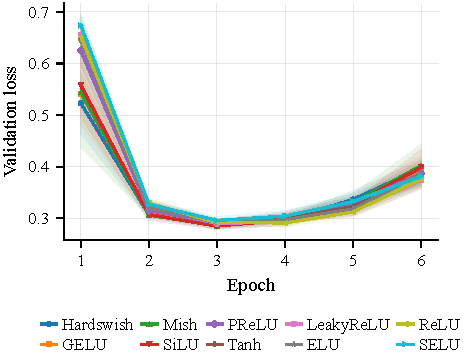
\includegraphics[width=0.92\columnwidth]{assets/convergence_curves.png}
  \caption{Per-Epoch Validation Accuracy (GRU, Homogeneous Pairs)}
  \label{fig:convergence_curves}
\end{figure}

\subsection{Prediction Balance Across Configurations}


Dropout(0.4) and gradient clipping ($L_2 \leq 1.0$) keep the worst
accuracy across all 400 models at 84.84\%, so no configuration
fails catastrophically. Finer differences appear in the precision--
recall gap, which measures whether the model treats both
classes equally. Table~\ref{tab:gen_balance} shows the five most balanced and
five most biased configurations across all four experiments.
The best case, SiLU + SELU in BiGRU+BiGRU, has a gap of
0.00\% (precision and recall both 87.60\%). The worst, Mish
+ GELU in BiGRU+BiGRU, has a gap of 11.71\% (precision
91.65\%, recall 79.94\%), meaning it predicts positive with
high confidence but misses roughly one in five actual positive
reviews. GRU-based experiments appear at both ends: they
produce the most balanced and the most biased configurations.

\begin{table}[htbp]
  \caption{Precision Recall Balance Across All 400 Configurations}
  \label{tab:gen_balance}
  \centering\footnotesize
  \renewcommand{\arraystretch}{1.05}
  \resizebox{\columnwidth}{!}{%
  \begin{tabular}{lcccc}
    \toprule
    Combination & Exp & Prec.\% & Rec.\% & P-R Gap\% \\
    \midrule
    \multicolumn{5}{l}{\textit{Most balanced}} \\
    SiLU + SELU        & BiGRU+BiGRU   & 87.60 & 87.60 & \textbf{0.00} \\
    PReLU + Tanh       & BiLSTM+BiLSTM & 86.60 & 86.62 & 0.02 \\
    Tanh + LeakyReLU   & BiGRU+GRU     & 87.23 & 87.26 & 0.03 \\
    GELU + SELU        & BiGRU+GRU     & 87.78 & 87.74 & 0.04 \\
    ReLU + GELU        & BiGRU+BiGRU   & 87.78 & 87.74 & 0.04 \\
    \midrule
    \multicolumn{5}{l}{\textit{Most biased}} \\
    Mish + GELU        & BiGRU+BiGRU   & 91.65 & 79.94 & \textbf{11.71} \\
    SELU + ELU         & BiGRU+GRU     & 90.88 & 79.32 & 11.56 \\
    Hardswish + Tanh   & BiGRU+GRU     & 90.76 & 79.76 & 11.00 \\
    Mish + Mish        & BiGRU+BiGRU   & 81.78 & 92.76 & 10.98 \\
    Hardswish + SiLU   & BiLSTM+BiLSTM & 82.53 & 92.68 & 10.15 \\
    \bottomrule
  \end{tabular}%
  }
\end{table}




\subsection{Computational Cost}

The 400 run study required approximately 98 GPU-minutes in total
on an NVIDIA RTX 5080. Table~\ref{tab:comp_cost} reports parameter
counts and training times. GRU models carry
approximately 3.8\% fewer parameters than their LSTM counterparts
due to the reduced gate count (three gates versus four).

\begin{table}[htbp]
  \caption{Computational Cost Summary}
  \label{tab:comp_cost}
  \centering\footnotesize
  \renewcommand{\arraystretch}{1.1}
  \resizebox{\columnwidth}{!}{%
  \begin{tabular}{lccc}
    \toprule
    Experiment & Params & Time/run & Total (100 runs) \\
    \midrule
    BiLSTM+LSTM    & ${\approx}$764K & ${\sim}$14\,s & ${\sim}$26 min \\
    BiGRU+GRU     & ${\approx}$734K & ${\sim}$13\,s & \textbf{21.4 min}$^{*}$ \\
    BiLSTM+BiLSTM & ${\approx}$787K & ${\sim}$15\,s & ${\sim}$27 min \\
    BiGRU+BiGRU  & ${\approx}$752K & ${\sim}$14\,s & ${\sim}$24 min \\
    \midrule
    \multicolumn{4}{l}{\textbf{Total (all 400 runs): ${\sim}$98 GPU-minutes}} \\
    \bottomrule
    \multicolumn{4}{l}{\small $^{*}$Directly measured on NVIDIA RTX 5080.}\\
    \multicolumn{4}{l}{\small All others estimated proportionally.}\\
    \multicolumn{4}{l}{\small Each run trains for ${\sim}$6 epochs (early stopping).}
  \end{tabular}%
  }
\end{table}





\FloatBarrier
\section{Discussion}
%------------------------------------------------------------------------------

\subsection{RQ1: Which Activation Pair Gives the Highest Accuracy?}

The highest accuracy across all 400 models is Tanh +
Hardswish in BiGRU+BiGRU at 88.06\% (F1 88.15\%). This
works because Tanh limits Dense Layer 1 outputs to the range
$(-1,1)$, and Hardswish is only zero for inputs below $-3$,
which Tanh outputs can never reach. The highest accuracy for
BiLSTM+LSTM is Mish + PReLU at 87.66\%. Looking at Act$_1$
averages (Table~\ref{tab:marginal}), Tanh and Mish are the two strongest Act$_1$
choices for BiLSTM+LSTM (86.95\% and 86.90\%), while for
BiGRU+GRU the leaders are ELU (87.69\%) and LeakyReLU
(87.60\%).

\begin{figure}[htbp]
  \centering
  \includegraphics[width=0.92\columnwidth]{assets/best_pairs.png}
  \caption{Highest-Accuracy Activation Pair per Architecture}
  \label{fig:best_pairs}
\end{figure}

\subsection{RQ2: Which Activation Converges Fastest?}
Table~\ref{tab:convergence} shows that Mish, Hardswish, and GELU reach
78 to 81\% validation accuracy after one epoch, while ReLU,
SELU, and LeakyReLU reach only 62 to 65\% under identical
conditions. SiLU belongs to the same smooth family as
Mish but starts at 71\%, comparable to ELU and PReLU,
so smoothness alone does not determine early convergence
speed. Hardswish, despite its dead zone for $x < -3$, is the
second fastest starter. After epoch 1 the differences narrow: all
functions reach their best validation loss at epoch 3 and trigger
early stopping at epoch 6. The fast starters do not produce
higher final accuracy; they reach comparable accuracy sooner.

\subsection{RQ3: Which Activation Produces the Most Balanced Predictions?}
The most balanced configuration across all 400 models
is SiLU + SELU in BiGRU+BiGRU, with a gap of 0.00\%
(precision and recall both 87.60\%). The most biased is Mish +
GELU in BiGRU+BiGRU, with a gap of 11.71\% (precision
91.65\%, recall 79.94\%). GRU-based architectures produce both
the most balanced and the most biased configurations, so GRU
is more stable in accuracy but not in prediction balance.

\subsection{RQ4: Does GRU React Differently than LSTM?}
Yes. GRU has a narrower accuracy range across all 100
activation pairs (2.37\% spread vs 2.82\% for LSTM) and a
higher mean accuracy (87.43\% vs 86.70\%, a gap of 0.73
points). A poor activation choice hurts GRU less than it hurts
LSTM. The preferred functions also differ: LSTM works best
with Tanh (86.95\%) and Mish (86.90\%) as Act$_1$ (Table~\ref{tab:marginal}),
while GRU works best with ELU (87.69\%) and LeakyReLU
(87.60\%).

Making both recurrent layers bidirectional has little effect.
BiLSTM+BiLSTM averages 86.79\%, only 0.09 points above
BiLSTM+LSTM (86.70\%), and BiGRU+BiGRU averages
87.30\%, actually 0.13 points below BiGRU+GRU (87.43\%).
The cell type (LSTM vs GRU) matters far more than whether
Layer 2 is bidirectional.

One pattern is consistent across both cell types: Tanh in the
Act$_2$ position, paired with certain Act$_1$ choices, produces the
worst results. ELU + Tanh reaches only 84.95\% in LSTM and
Hardswish + Tanh reaches only 85.82\% in GRU, both among
the lowest in their respective sweeps.

\subsection{RQ5: Do Non-Saturating Activations Improve Gradient Flow?}
Not always. In the BiLSTM+LSTM sweep, Tanh as Act$_1$
averages 86.95\% while ReLU averages 86.50\% (Table~\ref{tab:marginal}).
Tanh saturates and ReLU does not, yet Tanh wins by 0.45
points, because Tanh compresses LSTM's wide-range outputs
into a useful bounded range. In the BiGRU+GRU sweep the
situation reverses: ELU, a non-saturating function, leads as Act$_1$
at 87.69\% and appears in four of the top ten GRU configurations
(Table~\ref{tab:top_configs}). The answer is conditional. Non-saturating activations
help in GRU, where the outputs are already compact. In LSTM,
where outputs have higher variance, the range control of a
saturating function like Tanh can be more useful than the
gradient advantage of a non-saturating one.

\subsection{RQ6: Do ReLU-Based Dense Layers Exhibit Dead-Neuron Problems?}

Yes, and the effect is architecture-specific. ReLU + PReLU in
BiLSTM+LSTM achieves only 84.90\% (Table~\ref{tab:deadneuron}), the second
lowest result across all 400 models and 2.76 points below the
BiLSTM+LSTM peak. The same pair in BiGRU+GRU reaches
87.35\%, a gap of 2.45 points between the two architectures
using identical activation functions.

ReLU outputs zero for any negative input, and its gradient
is also zero, so the neuron stops learning permanently. In
Dense Layer 1, if the values from the recurrent layer are
mostly negative for some neurons, those neurons die and never
recover. Dense Layer 2 then receives near-zero inputs from the
dead neurons. When Dense Layer 2 uses PReLU, it gets no
useful gradient from those inputs and cannot adapt its learnable
slope, so the dense layers lose capacity. This does not happen
in GRU, whose outputs are more evenly distributed, so fewer
neurons die. Table~\ref{tab:deadneuron} shows the pattern across different Act$_2$
choices when ReLU is fixed as Act$_1$: LeakyReLU in Act$_2$
recovers most of the lost accuracy (87.56\%) because it passes
small negative values instead of zeroing them out.

\begin{table}[htbp]
  \caption{ReLU as Act$_1$: Effect of Different Act$_2$ Choices}
  \label{tab:deadneuron}
  \centering\footnotesize
  \setlength{\tabcolsep}{3pt}
  \renewcommand{\arraystretch}{1.08}
  \resizebox{\columnwidth}{!}{%
  \begin{tabular}{lccc}
    \toprule
    Combination & BiLSTM+LSTM & BiGRU+GRU & Gap \\
    \midrule
    ReLU + PReLU     & 84.90 & 87.35 & 2.45 \\
    ReLU + Tanh      & 85.56 & ---   & --- \\
    ReLU + GELU      & 86.52 & ---   & --- \\
    ReLU + ReLU      & 86.59 & 87.34 & 0.75 \\
    ReLU + LeakyReLU & 87.56 & ---   & --- \\
    \bottomrule
  \end{tabular}%
  }
\end{table}

\FloatBarrier


\section{Conclusion}

This study tested all 100 ordered pairs of the ten activation
functions in Table~\ref{tab:activations} across four gated recurrent architectures
(400 models total) on the IMDb dataset~\cite{maas2011}, with every other
setting held fixed.

Seven findings follow from the data. First, the highest
accuracy across all 400 models is Tanh + Hardswish in
BiGRU+BiGRU at 88.06\% (Table~\ref{tab:top_configs}). Second, GRU-based
architectures outperform LSTM by 0.73 points on average
(87.43\% vs 86.70\%) with a narrower accuracy spread (2.37\%
vs 2.82\%), so GRU is less affected by a poor activation
choice; making both layers bidirectional changes little (BiLSTM+BiLSTM
is only 0.09 points above BiLSTM+LSTM, and
BiGRU+BiGRU is 0.13 points below BiGRU+GRU), so the
cell type matters more than bidirectionality. Third, activation
rankings invert between architectures: ELU is the best Act$_1$ for
GRU but the worst for LSTM, and Tanh is the best for LSTM
but seventh for GRU, so rankings from one architecture do
not transfer to another. Fourth, Mish, Hardswish, and GELU
reach 78 to 81\% validation accuracy after one epoch while
ReLU and SELU reach only 62 to 64\% (Table~\ref{tab:convergence}), although
all functions converge to comparable final accuracy by epoch 3.
Fifth, cross-function pairs produce the highest peak accuracy in
every experiment, but same-function pairs have equal or slightly
higher mean accuracy in two of the four sweeps. Sixth, using
ReLU as Act$_1$ in BiLSTM+LSTM dense layers causes dead
neurons: ReLU + PReLU drops to 84.90\%, while the same
pair in BiGRU+GRU reaches 87.35\% (Table~\ref{tab:deadneuron}), confirming
an architecture-specific failure. Seventh, no configuration in
the single-seed sweep beat the 88.40\% benchmark, but Mish
and SiLU reached 88.48\% and 88.43\% under a different seed
in the convergence rerun, showing the benchmark sits within
normal seed variance.

Future work should test whether these findings hold on
other sentiment datasets, investigate activation function choice
inside attention mechanisms, and run multi-seed experiments to
measure how much results vary across random initializations.

\begin{thebibliography}{23}

% -- Gated Recurrent Architectures --

\bibitem{hochreiter1997}
S. Hochreiter and J. Schmidhuber,
``Long short-term memory,''
\textit{Neural Computation}, vol.~9, no.~8, pp.~1735--1780, Nov. 1997.

\bibitem{cho2014}
K. Cho, B. van Merri\"{e}nboer, C. Gulcehre, D. Bahdanau, F. Bougares,
H. Schwenk, and Y. Bengio,
``Learning phrase representations using RNN encoder-decoder for statistical
machine translation,''
in \textit{Proc. EMNLP}, 2014, pp.~1724--1734.

\bibitem{chung2014}
J. Chung, C. Gulcehre, K. Cho, and Y. Bengio,
``Empirical evaluation of gated recurrent neural networks on sequence
modeling,''
\textit{arXiv preprint arXiv:1412.3555}, 2014.

\bibitem{schuster1997}
M. Schuster and K.~K. Paliwal,
``Bidirectional recurrent neural networks,''
\textit{IEEE Trans. Signal Process.}, vol.~45, no.~11,
pp.~2673--2681, Nov. 1997.

% -- Activation Functions --

\bibitem{nair2010}
V. Nair and G.~E. Hinton,
``Rectified linear units improve restricted Boltzmann machines,''
in \textit{Proc. ICML}, 2010, pp.~807--814.

\bibitem{maas2013}
A.~L. Maas, A.~Y. Hannun, and A.~Y. Ng,
``Rectifier nonlinearities improve neural network acoustic models,''
in \textit{Proc. ICML Workshop on Deep Learning for Audio, Speech and
Language Processing}, 2013.

\bibitem{he2015}
K. He, X. Zhang, S. Ren, and J. Sun,
``Delving deep into rectifiers: Surpassing human-level performance on
ImageNet classification,''
in \textit{Proc. ICCV}, 2015, pp.~1026--1034.

\bibitem{clevert2015}
D. Clevert, T. Unterthiner, and S. Hochreiter,
``Fast and accurate deep network learning by exponential linear units
(ELUs),''
\textit{arXiv preprint arXiv:1511.07289}, 2015.

\bibitem{klambauer2017}
G. Klambauer, T. Unterthiner, A. Mayr, and S. Hochreiter,
``Self-normalizing neural networks,''
in \textit{Proc. NeurIPS}, 2017, pp.~971--980.

\bibitem{hendrycks2016}
D. Hendrycks and K. Gimpel,
``Gaussian error linear units (GELUs),''
\textit{arXiv preprint arXiv:1606.08415}, 2016.

\bibitem{ramachandran2017}
P. Ramachandran, B. Zoph, and Q.~V. Le,
``Searching for activation functions,''
\textit{arXiv preprint arXiv:1710.05941}, 2017.

\bibitem{misra2020}
D. Misra,
``Mish: A self regularized non-monotonic activation function,''
in \textit{Proc. BMVC}, 2020.

\bibitem{howard2019}
A. Howard \textit{et al.},
``Searching for MobileNetV3,''
in \textit{Proc. ICCV}, 2019, pp.~1314--1324.

\bibitem{apicella2021}
A. Apicella, F. Donnarumma, F. Isgr\`{o}, and R. Prevete,
``A survey on modern trainable activation functions,''
\textit{Neural Networks}, vol.~138, pp.~14--32, 2021.

\bibitem{nwankpa2018}
C. Nwankpa, W. Ijomah, A. Gachagan, and S. Marshall,
``Activation functions: Comparison of trends in practice and research for
deep learning,''
\textit{arXiv preprint arXiv:1811.03378}, 2018.

% -- Sentiment Analysis --

\bibitem{maas2011}
A.~L. Maas, R.~E. Daly, P.~T. Pham, D. Huang, A.~Y. Ng, and C. Potts,
``Learning word vectors for sentiment analysis,''
in \textit{Proc. ACL}, 2011, pp.~142--150.

\bibitem{ahmed2025}
S.~A. Ahmed \textit{et al.},
``Comparative analysis of activation functions in LSTM models for sentiment
classification,''
\textit{IJARCCE}, vol.~14, no.~4, Apr. 2025.

\bibitem{zhu2022}
Y. Zhu and R. Tan,
``A novel activation function based recurrent neural networks and their
applications on sentiment classification and log anomaly detection,''
\textit{Frontiers in Neurorobotics}, vol.~16, 2022.

\bibitem{socher2013}
R. Socher, A. Perelygin, J. Wu, J. Chuang, C.~D. Manning, A. Ng,
and C. Potts,
``Recursive deep models for semantic compositionality over a sentiment
treebank,''
in \textit{Proc. EMNLP}, 2013, pp.~1631--1642.

\bibitem{tang2015}
D. Tang, B. Qin, and T. Liu,
``Document modeling with gated recurrent neural network for sentiment
classification,''
in \textit{Proc. EMNLP}, 2015, pp.~1422--1432.

% -- Direct Competitors --

\bibitem{eger2018}
S. Eger, P. Youssef, and I. Gurevych,
``Is it time to swish? Comparing deep learning activation functions across
NLP tasks,''
in \textit{Proc. EMNLP}, 2018, pp.~4423--4433.

\bibitem{farzad2019}
A. Farzad, H. Mashayekhi, and H. Hassanpour,
``A comparative performance analysis of different activation functions in
LSTM networks for classification,''
\textit{Neural Computing and Applications}, vol.~31,
pp.~2507--2521, 2019.

\bibitem{essaiAli2022}
M.~H. Essai~Ali, A.~I. Taloba, M.~F. Farhan, and R.~A. Abozeid,
``Developing novel activation functions based deep learning LSTM for
classification,''
\textit{IEEE Access}, vol.~10, pp.~96578--96591, 2022.

\end{thebibliography}
\end{document}
